%-----------------------------------------------------------------------------------------------
\makeatletter
\immediate\write18{datelog > \jobname.info} % site script for $(date '+%Y-%m-%d %Hh%Mm%Ss')
\makeatother
%-----------------------------------------------------------------------------------------------
%-----------------------------------------------------------------------------------------------
\usetheme{Copenhagen}
\usepackage{beamercolorthemeCNThermSci2}
\usefonttheme{serif}
%-----------------------------------------------------------------------------------------------

%-----------------------------------------------------------------------------------------------
%-----------------------------------------------------------------------------------------------
\usetheme{Copenhagen}
\usepackage{beamercolorthemeUTF2}
\usefonttheme{serif}
%-----------------------------------------------------------------------------------------------
\usepackage[utf8]{inputenc}
\usepackage[greek,french,english,brazil]{babel} % last becomes the active one
\usepackage{pslatex}
\usepackage{amssymb,amsmath}
\usepackage{soul}
\usepackage[squaren,Gray]{SIunits}
\usepackage[nice]{nicefrac}
\usepackage{tikz}
\usepackage{xspace}
%-----------------------------------------------------------------------------------------------


%-----------------------------------------------------------------------------------------------
%-----------------------------------------------------------------------------------------------
% Mathematical
%-----------------------------------------------------------------------------------------------
\newcommand{\vet}[1]{\underline{{#1}}}
\newcommand{\mat}[1]{\underline{\underline{{#1}}}}
\newcommand{\cub}[1]{\underline{\underline{\underline{{#1}}}}}
\newcommand{\eqdef}{{\ensuremath\stackrel{\text{\tiny def}}{=}}}
%-----------------------------------------------------------------------------------------------
% Presentation
%-----------------------------------------------------------------------------------------------
\newcommand{\BkgImgH}[1]{% Places an image centered on the slide background filling the height
    \usebackgroundtemplate{\parbox{\paperwidth}{%
        \vspace*{1sp}\centering\includegraphics[height=\paperheight]{{#1}}
}}}
\newcommand{\BkgImgW}[1]{% Places an image centered on the slide background filling the width
    \usebackgroundtemplate{\parbox{\paperwidth}{%
        \vspace*{1sp}\centering\includegraphics[width=\paperwidth]{{#1}}
}}}
\newcommand{\ArtEndH}[3]{% Transitions to plain image (last) slide: #1:prefix #2,#3:extensions
    \BkgImgH{root/../art/#1.#2}
    \frame[plain]<handout:0>{%
        \transdissolve\vspace*{80mm}\color{white}\bf\input{root/../art/#1.#3}
}}
\newcommand{\ArtEndW}[3]{% Transitions to plain image (last) slide: #1:prefix #2,#3:extensions
    \BkgImgW{root/../art/#1.#2}
    \frame[plain]<handout:0>{%
        \transdissolve\vspace*{80mm}\color{white}\bf\input{root/../art/#1.#3}
}}
\newcommand{\ImgColW}[3]{% Inserts a full-width image in a column
    \includegraphics[width=\columnwidth]{root/../art/#1.#2}\\[-0.5\baselineskip]
    \parbox{\columnwidth}{\tiny\hfill\scalebox{0.65}{\input{root/../art/#1.#3}}}
}
\newcommand{\txtpic}[1]{%
    \fcolorbox{lightgray}{white!90!black}{{#1}} 
}
%-----------------------------------------------------------------------------------------------


%-----------------------------------------------------------------------------------------------
\newcommand{\VPMS}{{\ensuremath V_{\mathrm{PMS}}}}
\newcommand{\VPMI}{{\ensuremath V_{\mathrm{PMI}}}}
%-----------------------------------------------------------------------------------------------
\title{B.01.02 -- Ciclos de Potência Padrão a Ar}
\subtitle{Básico de Motores Alternativos}
\author{Prof.~C.~Naaktgeboren, PhD}
\date{{\scriptsize\tt%
    \includegraphics[height=6.0mm]{cc/by-nc-nd-88x31.pdf}\\[\smallskipamount]
    https://github.com/CNThermSci/ApplThermSci\\
    Compiled on \input{\jobname.info}
}}
%-----------------------------------------------------------------------------------------------
\begin{document}
%-----------------------------------------------------------------------------------------------
\logo{%
    \parbox{158mm}{% There's a 1mm gap on each side of the 160mm x 90mm slide logo line
        \mode<beamer>{
            \includegraphics[height=6.0mm]{root/00-res/UTFPR/UTFPR-logo-D.pdf}\hfill%
            
\includegraphics[height=9.0mm]{root/00-res/logo/CNThermSci-logo-A.pdf}%
        }
        \mode<handout>{
            
\includegraphics[height=6.0mm]{root/00-res/UTFPR/UTFPR-logo-W.pdf}\hfill%
            
\includegraphics[height=9.0mm]{root/00-res/logo/CNThermSci-logo-W.pdf}%
        }
    }
} % The (delineated, alpha), or washed-out logos
%-----------------------------------------------------------------------------------------------
\frame{\titlepage}
%-----------------------------------------------------------------------------------------------

%-----------------------------------------------------------------------------------------------
\frame{\tableofcontents}
%-----------------------------------------------------------------------------------------------

%-----------------------------------------------------------------------------------------------
\section{Básico de Motores Alternativos}
%-----------------------------------------------------------------------------------------------

    \begin{frame}
        \vspace*{-0.35cm}
        \figfigW{fig/MotoresAlt-01.pdf}
    \end{frame}

    % !j 96 -i8
    %-------------------------------------------------------------------------------------------
    \begin{frame}
        \begin{columns}
        \column{0.70\textwidth}
            \begin{align*}
                \uncover<1->{
                    \alert{r} &
                    = \frac{V_\mathrm{max}}{V_\mathrm{min}}
                    \alert{= \frac{\VPMI}{\VPMS}},
                    \\[\bigskipamount]
                }
                \uncover<2->{
                    \alert{V_\mathrm{du}} &
                    = V_\mathrm{max} - V_\mathrm{min}
                    \alert{= \VPMI - \VPMS},
                    \qquad\mbox{e}
                    \\[\bigskipamount]
                }
                \uncover<3->{
                    \alert{\eta_t} &
                    \alert{= \frac{W_\mathrm{liq}}{Q_\mathrm{liq}}}
                    = \frac{w_\mathrm{liq}}{q_\mathrm{liq}}.
                }
            \end{align*}
        \column{0.30\textwidth}
            \figfigW{fig/MotoresAlt-02.pdf}
        \end{columns}
    \end{frame}
    %-------------------------------------------------------------------------------------------

    % !j 96 -i8
    %-------------------------------------------------------------------------------------------
    \begin{frame}
        \begin{center}
            \begin{figure}
                \fontsize{3.0}{4}\selectfont
                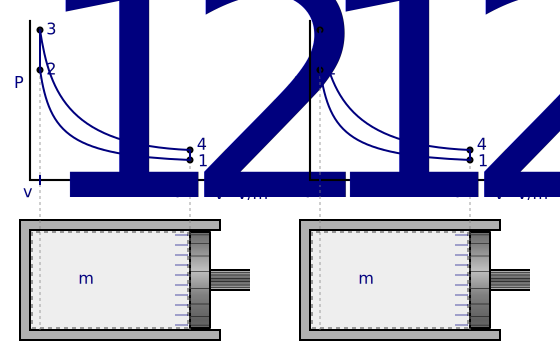
\includegraphics[height=0.7\textheight]{fig/MotoresAlt-PME.pdf}
                \\\vspace*{-2.5em}\texttt{autoria própria}
            \end{figure}
        \end{center}
        \begin{align*}
            \alert{\mathrm{PME}} &
            = \frac{W_\mathrm{liq}}{V_\mathrm{du}}
            \alert{= \frac{W_\mathrm{liq}}{\VPMI - \VPMS}}
            = \frac{W_\mathrm{liq}}{\VPMS(r-1)}.
        \end{align*}
    \end{frame}
    %-------------------------------------------------------------------------------------------

%-----------------------------------------------------------------------------------------------
\section{Tópicos de Leitura}
%-----------------------------------------------------------------------------------------------

    %------------------------------------------------------------------------------------------
    \begin{frame}[allowframebreaks]{Tópicos de Leitura}
        \begin{thebibliography}{Çengel, Y.~A., 2013}
            \bibitem[Çengel, Y.~A., 2013]{2013-CengelYA+BolesMA-AMGH}
                Çengel, Y.~A. e Boles, M.~A.
                \newblock{%
                    {\em Termodinâmica $7^\mathrm{a}\!$ Edição\/}.
                    \alert{Seção~9-4.}
                }
                \newblock{\footnotesize AMGH. Porto Alegre. ISBN 978-85-8055-200-3.}
        \end{thebibliography}
    \end{frame}
    %------------------------------------------------------------------------------------------

    % Finishes with stunning image, with credit
    \ArtEndW{pexels-matt-hardy-1533720}{jpg}{txt}

%-----------------------------------------------------------------------------------------------
\end{document}
%-----------------------------------------------------------------------------------------------

